\documentclass[11pt,a4paper]{article}
\usepackage[margin=2.4cm]{geometry}
\usepackage{amsmath,amssymb,bm}
\usepackage{booktabs}
\usepackage{siunitx}
\usepackage{enumitem}
\usepackage{graphicx}
\graphicspath{{matlab/figs/}}
\usepackage[hidelinks]{hyperref}

\sisetup{detect-all}
\newcommand{\dd}{\mathrm{d}}
\newcommand{\T}{^{\top}}
\newcommand{\df}{\delta_f}
\newcommand{\dr}{\delta_r}
\newcommand{\half}{\tfrac{1}{2}}

\title{Ride-Height and Pitch Dynamics of a Fully Submerged Hydrofoil Boat:\\
Nonlinear Model, Trim and LTI State-Space Form}
\author{ELEC3304 Control --- Practical Week 9 / Assessment 2\\[2pt]
Group members: \emph{(name 1)}, \emph{(name 2)}}
\date{October 2026}

\begin{document}
\maketitle

\section{System and control objective}

The plant is a small single-seat hydrofoil boat of the solar-boat class, with
parameters taken from the T\'ecnico Solar Boat SR02 \cite{belime}. Above its
take-off speed the hull is carried clear of the water by three fully submerged
foils: two at the front (port and starboard, treated here as one lifting surface)
and one at the rear on the propulsion strut.

A fully submerged foil, unlike a surface-piercing one, has almost no natural
tendency to return to a given depth: its lift is nearly independent of how deep
it runs. The boat therefore cannot hold a ride height by itself and needs active
control \cite{belime}. The control objective is to regulate the ride height at a
set value and keep the hull level, in the presence of waves, using only small
changes of the foil incidence angles.

We consider the longitudinal (vertical-plane) motion only: heave and pitch.

\section{Signals}

\begin{table}[h]
\centering
\begin{tabular}{@{}llp{8.4cm}l@{}}
\toprule
Role & Symbol & Meaning & Unit \\ \midrule
State & $h$ & heave: height of the centre of mass (CM) above its trim height, positive up & \si{m} \\
State & $v=\dot h$ & vertical velocity of the CM, positive up & \si{m/s} \\
State & $\theta$ & pitch angle, positive bow-up & \si{rad} \\
State & $q=\dot\theta$ & pitch rate & \si{rad/s} \\
Input & $\df$ & incidence of the front foils relative to the hull & \si{rad} \\
Input & $\dr$ & incidence of the rear foil relative to the hull & \si{rad} \\
Output & $y_1$ & ride height measured by an ultrasonic sensor at the bow & \si{m} \\
Output & $y_2$ & pitch angle measured by an attitude reference unit (AHRS) & \si{rad} \\
Output & $y_3$ & pitch rate measured by a rate gyro & \si{rad/s} \\
Disturbance & $w_f,\,w_r$ & vertical water velocity (wave orbital motion) at the front / rear foil & \si{m/s} \\
Disturbance & $n_1,\,n_2,\,n_3$ & measurement noise; $n_1$ also contains the wave elevation under the height sensor & \si{m}, \si{rad}, \si{rad/s} \\
\bottomrule
\end{tabular}
\end{table}

There are $n_x=4$ states, $n_u=2$ actuators and $n_y=3$ sensors, so the system has
fewer measurements than states and the unmeasured states must be estimated. The
sensors are the ones fitted to the real boat \cite{belime}: an ultrasonic height
sensor at the bow and an attitude and heading reference system (AHRS), which
provides both the pitch angle and the pitch rate. Heave and heave rate are not
measured; the choice of sensors is justified in Section~\ref{sec:obsv}.

\section{Modelling assumptions}
\label{sec:assumptions}

\begin{enumerate}[label=A\arabic*.,leftmargin=2.6em]
\item The boat is foil-borne; the hull does not touch the water.
\item Motion is confined to the vertical plane. Roll, sway and yaw are zero.
\item The forward speed $U$ is constant. On the real boat a separate speed loop
      acts on the throttle \cite{belime}; variations of $U$ are treated as model
      uncertainty in Section~\ref{sec:uncertainty}.
\item Foil drag and propeller thrust are neglected in the heave and pitch
      equations. At trim they cancel in the surge direction and their net pitching
      moment is about $\SI{20}{N.m}$, roughly \SI{1}{\percent} of the
      $\SI{1600}{N.m}$ moment of each foil group about the CM. The change of
      drag with angle of attack is a few percent of the change of lift.
\item Foil lift is quasi-steady, with a lift coefficient that is affine in the
      angle of attack, $C_L(\alpha)=C_{L0}+C_{L\alpha}\alpha$, valid below stall
      ($|\alpha|\lesssim\SI{12}{\degree}$, assumed).
\item Hydrodynamic added mass of the foils is neglected. Estimated as
      $\tfrac{\pi}{4}\rho c^2 b$ per foil it totals about \SI{8}{kg}, i.e.\
      \SI{4}{\percent} of the boat mass.
\item The front foils move together (common mode). The rear foil is assumed to be
      actuated; on SR02 it was fixed and its actuation was listed as future work
      \cite{belime}.
\item Actuator dynamics are neglected in the design model; position and rate
      limits are kept as constraints (Section~\ref{sec:constraints}). In
      simulation each foil actuator is modelled as a position limit, a
      first-order servo lag with time constant $\tau_a$, and a rate limit.
\end{enumerate}

\section{Nonlinear model}

\subsection{Kinematics}

Each foil group $i\in\{f,r\}$ is located, in hull axes, a distance $x_i$ ahead of
the CM and $z_i$ below it, with $x_f=l_f>0$ and $x_r=-l_r<0$. The foils sit well
below the CM, so $z_i$ cannot be ignored. When the hull is pitched by $\theta$ the
foil position relative to the CM, in horizontal/vertical axes, is
\begin{equation}
X_i = x_i\cos\theta + z_i\sin\theta, \qquad
Z_i = x_i\sin\theta - z_i\cos\theta .
\label{eq:pos}
\end{equation}
Differentiating, and subtracting the vertical water velocity $w_i$, gives the
velocity of each foil relative to the water:
\begin{equation}
u_i = U + q\,(z_i\cos\theta - x_i\sin\theta), \qquad
v_i = v + q\,X_i - w_i .
\label{eq:vfoil}
\end{equation}
The inflow angle is $\gamma_i=\arctan(v_i/u_i)$. A foil that moves upward sees the
flow coming from above, which reduces its angle of attack:
\begin{equation}
\alpha_i = \delta_i + \theta - \gamma_i .
\label{eq:alpha}
\end{equation}
The term $-\gamma_i$ is what provides heave and pitch damping. It is absent from
the model of \cite{belime}, which uses $\alpha=\delta+\theta$; we follow
\cite{renyang,liu} and keep it.

With $d_0$ the submergence of the foils at trim, the instantaneous submergence is
\begin{equation}
d_i = d_0 - h - x_i\sin\theta - z_i\,(1-\cos\theta) .
\label{eq:depth}
\end{equation}

\subsection{Foil lift with free-surface effect}

The lift of foil group $i$ with planform area $S_i$ is
\begin{equation}
L_i = \half\,\rho\,\bigl(u_i^2+v_i^2\bigr)\,S_i\;K\!\left(\frac{d_i}{c}\right)
      \bigl(C_{L0}+C_{L\alpha}\,\alpha_i\bigr),
\label{eq:lift}
\end{equation}
where $c$ is the foil chord and $K$ accounts for the loss of lift near the free
surface. For the high Froude numbers at which hydrofoils operate we use the
infinite-Froude-number (``biplane'') result of linear theory, derived in
Appendix~\ref{app:K} (see also \cite{faltinsen}, ch.~6),
\begin{equation}
K(\xi)=\frac{1+16\,\xi^{2}}{2+16\,\xi^{2}}, \qquad
K'(\xi)=\frac{32\,\xi}{\bigl(2+16\,\xi^{2}\bigr)^{2}}, \qquad \xi=\frac{d}{c}.
\label{eq:K}
\end{equation}
$K\to1$ for a deeply submerged foil and $K\to\half$ as the foil reaches the
surface. Because $K'>0$, a boat that rises loses lift, which gives a (weak)
restoring force in heave.

\subsection{Equations of motion}

Lift acts perpendicular to the relative flow, so foil $i$ applies the force
$(-L_i\sin\gamma_i,\;L_i\cos\gamma_i)$ at the point $(X_i,Z_i)$. Newton's second
law in the vertical direction and about the pitch axis gives
\begin{align}
m\,\dot v &= \sum_{i\in\{f,r\}} L_i\cos\gamma_i \;-\; m g, \label{eq:heave}\\
I_y\,\dot q &= \sum_{i\in\{f,r\}} L_i\,\bigl(X_i\cos\gamma_i + Z_i\sin\gamma_i\bigr),
\label{eq:pitch}
\end{align}
together with $\dot h=v$ and $\dot\theta=q$. With
$\bm x=[\,h\;\;v\;\;\theta\;\;q\,]\T$, $\bm u=[\,\df\;\;\dr\,]\T$ and
$\bm w=[\,w_f\;\;w_r\,]\T$ this is a nonlinear system
$\dot{\bm x}=\bm f(\bm x,\bm u,\bm w)$. The nonlinearities are the trigonometric
terms, the dependence of dynamic pressure on the foil velocity, the free-surface
factor $K$, and (in simulation) stall and actuator saturation.

\subsection{Measurement}

The ultrasonic sensor is mounted a distance $l_s$ ahead of the CM and measures
the height of the bow above the water; the AHRS measures the pitch angle and the
pitch rate. Relative to the trim readings,
\begin{equation}
y_1 = h + l_s\sin\theta + n_1, \qquad y_2 = \theta + n_2, \qquad y_3 = q + n_3 .
\label{eq:meas}
\end{equation}
The height sensor sees a mixture of heave and pitch, not either state alone, and
its reading is corrupted by the wave surface passing under the bow.

\section{Parameters}

\begin{table}[h]
\centering
\begin{tabular}{@{}llll@{}}
\toprule
Symbol & Description & Value & Source \\ \midrule
$m$ & mass of boat and pilot & \SI{215}{kg} & \cite{belime} \\
$I_y$ & pitch moment of inertia & \SI{503}{kg.m^2} & \cite{belime} \\
$S_f$ & front foil area ($2\times\SI{0.048}{m^2}$) & \SI{0.096}{m^2} & \cite{belime} \\
$S_r$ & rear foil area & \SI{0.046}{m^2} & \cite{belime} \\
$l_f$ & CM to front foils & \SI{1.10}{m} & \cite{belime} \\
$l_r$ & CM to rear foil & \SI{2.45}{m} & \cite{belime} \\
$z_f$ & front foils below CM & \SI{0.75}{m} & \cite{belime} \\
$z_r$ & rear foil below CM & \SI{0.96}{m} & \cite{belime} \\
$l_s$ & CM to ultrasonic sensor & \SI{3.0}{m} & \cite{belime} \\
$C_{L0}$ & lift coefficient at zero incidence (NACA 63-412) & 0.288 & \cite{belime} \\
$C_{L\alpha}$ & lift-curve slope, $0.090$ per degree & \SI{5.157}{rad^{-1}} & \cite{belime} \\
$U_0$ & cruise speed & \SI{7}{m/s} & \cite{belime} \\
$\rho$ & sea-water density & \SI{1025}{kg/m^3} & \cite{belime} \\
$g$ & gravitational acceleration & \SI{9.81}{m/s^2} & --- \\
$c$ & foil chord & \SI{0.073}{m} & estimated$^{\ast}$ \\
$d_0$ & foil submergence at trim & \SI{0.30}{m} & assumed$^{\dagger}$ \\
$\alpha_{\mathrm{stall}}$ & angle of attack beyond which lift stops rising & \SI{12}{\degree} & assumed \\
$\tau_a$ & servo time constant (simulation only) & \SI{0.02}{s} & assumed \\
$\sigma_y$ & height sensor noise, std & \SI{1}{cm} & assumed \\
$\sigma_\theta$ & AHRS pitch-angle noise, std & \SI{0.3}{\degree} & assumed \\
$\sigma_q$ & rate gyro noise, std & \SI{0.2}{\degree/s} & assumed \\
\bottomrule
\end{tabular}
\end{table}

\noindent$^{\ast}$\,Not reported in \cite{belime}. The reported slope
$0.090$/deg, with the finite-span correction $C_L=C_l\,\mathrm{AR}/(\mathrm{AR}+2)$
used there and a section slope of $2\pi\ \mathrm{rad^{-1}}$, implies an aspect ratio
$\mathrm{AR}\approx9$, hence $c=\sqrt{S/\mathrm{AR}}\approx\SI{0.073}{m}$ for one
front foil.\\
$^{\dagger}$\,Not reported. Chosen so that the foils run about four chords deep
with the hull $0.3$--$\SI{0.4}{m}$ above the water. Its effect is examined in
Section~\ref{sec:uncertainty}.

\section{Equilibrium (trim)}

We look for a steady level flight condition in calm water:
$\bm x_0=\bm 0$, $\bm w=\bm 0$, $U=U_0$. Setting $\dot v=\dot q=0$ in
\eqref{eq:heave}--\eqref{eq:pitch} gives a force and a moment balance,
\[
L_{f0}+L_{r0}=mg, \qquad l_f L_{f0}=l_r L_{r0},
\]
so the weight is shared in inverse proportion to the lever arms:
\begin{equation}
L_{f0}=\frac{l_r}{l_f+l_r}\,mg=\SI{1455.6}{N}, \qquad
L_{r0}=\frac{l_f}{l_f+l_r}\,mg=\SI{653.5}{N}.
\end{equation}
Inverting \eqref{eq:lift} with $u_i=U_0$, $v_i=0$ gives the trim incidences in closed form:
\begin{equation}
\delta_{i0}=\frac{1}{C_{L\alpha}}
\left(\frac{L_{i0}}{\half\rho U_0^2 S_i K_0}-C_{L0}\right),
\qquad K_0=K(d_0/c)=0.9963 ,
\label{eq:trim}
\end{equation}
which yields $\delta_{f0}=\SI{3.53}{\degree}$ and $\delta_{r0}=\SI{3.11}{\degree}$
at $U_0=\SI{7}{m/s}$.

\paragraph{Validation.} Table~\ref{tab:trim} compares \eqref{eq:trim} with the
trim angles that \cite{belime} obtained numerically from a model that includes
drag and thrust. The agreement supports assumption~A4.

\begin{table}[h]
\centering
\caption{Trim incidences versus speed: this model and \cite{belime}.}
\label{tab:trim}
\begin{tabular}{@{}ccccc@{}}
\toprule
$U$ (\si{m/s}) & $\delta_{f0}$ (deg) & $\delta_{f0}$ \cite{belime} &
$\delta_{r0}$ (deg) & $\delta_{r0}$ \cite{belime} \\ \midrule
6  & 5.97 & 5.9 & 5.39 & 5.5 \\
7  & 3.53 & 3.5 & 3.11 & 3.2 \\
8  & 1.96 & 1.9 & 1.63 & 1.7 \\
9  & 0.87 & 0.8 & 0.62 & 0.7 \\
10 & 0.10 & 0.1 & $-0.11$ & 0.0 \\
\bottomrule
\end{tabular}
\end{table}

\section{Linearisation}

Define deviations from trim, $\tilde{\bm u}=\bm u-\bm u_0$ (the states and
disturbances are already zero at trim). To first order,
\[
X_i\approx x_i+z_i\theta,\quad Z_i\approx -z_i,\quad
u_i\approx U_0+z_i q,\quad
\gamma_i\approx\frac{v+x_i q-w_i}{U_0},\quad
d_i\approx d_0-h-x_i\theta .
\]
The lift perturbation of foil group $i$ is therefore
\begin{equation}
\tilde L_i = k_i\Bigl(\tilde\delta_i+\theta-\frac{v+x_i q-w_i}{U_0}\Bigr)
             -\kappa_i\,(h+x_i\theta) + \sigma_i\,q ,
\label{eq:Ltilde}
\end{equation}
with three coefficients per foil group,
\begin{equation}
k_i=\left.\frac{\partial L_i}{\partial\alpha_i}\right|_0
   =\half\rho U_0^2 S_i K_0 C_{L\alpha},
\qquad
\kappa_i=\left.\frac{\partial L_i}{\partial d_i}\right|_0
   =\frac{L_{i0}}{c}\,\frac{K'(d_0/c)}{K_0},
\qquad
\sigma_i=\left.\frac{\partial L_i}{\partial u_i}\right|_0 z_i
   =\frac{2L_{i0}z_i}{U_0}.
\end{equation}
Here $k_i$ is the lift per unit angle of attack, $\kappa_i$ the lift gained per
metre of extra submergence, and $\sigma_i$ the lift gained because a pitch rate
moves a foil below the CM forward through the water. Numerically
$k_f=\SI{12386}{N/rad}$, $k_r=\SI{5935}{N/rad}$,
$\kappa_f=\SI{35.5}{N/m}$, $\kappa_r=\SI{15.9}{N/m}$,
$\sigma_f=\SI{312}{N.s/rad}$ and $\sigma_r=\SI{179}{N.s/rad}$.

Linearising \eqref{eq:heave} and \eqref{eq:pitch}, and using the trim balance
$\sum_i L_{i0}x_i=0$, gives
\begin{align}
m\,\dot v &= \sum_i \tilde L_i, \\
I_y\,\dot q &= \sum_i x_i\tilde L_i
   \;+\; W_z\,\theta \;-\; \sum_i L_{i0}z_i\,\frac{v+x_i q-w_i}{U_0},
\qquad W_z=\sum_i L_{i0}z_i=\SI{1719}{N.m}.
\label{eq:pitchlin}
\end{align}
The last two terms of \eqref{eq:pitchlin} come from the vertical offset of the
foils. $W_z\theta$ is an inverted-pendulum moment: the weight is carried at points
below the CM, so pitching the hull moves the lift forward. The final term is the
moment of the backward tilt of the lift vector when a foil rises. The two cancel
when the boat climbs along its own axis ($v=U_0\theta$), as they must.

Collecting terms gives the LTI model
\begin{equation}
\dot{\bm x}=A\bm x+B\tilde{\bm u}+E\bm w, \qquad y=C\bm x+D\tilde{\bm u}+n,
\end{equation}
\begin{equation}
A=\begin{bmatrix}
0 & 1 & 0 & 0\\[4pt]
-\dfrac{\sum\kappa_i}{m} &
-\dfrac{\sum k_i}{mU_0} &
\dfrac{\sum (k_i-\kappa_i x_i)}{m} &
\dfrac{\sum(\sigma_i-k_i x_i/U_0)}{m}\\[10pt]
0 & 0 & 0 & 1\\[4pt]
-\dfrac{\sum\kappa_i x_i}{I_y} &
-\dfrac{\sum k_i x_i + W_z}{I_yU_0} &
\dfrac{\sum (k_i x_i-\kappa_i x_i^2)+W_z}{I_y} &
-\dfrac{\sum (k_i x_i^2-L_{i0}z_i x_i)}{I_yU_0}
\end{bmatrix},
\label{eq:Asym}
\end{equation}
\begin{equation}
B=\begin{bmatrix}
0 & 0\\[2pt]
\dfrac{k_f}{m} & \dfrac{k_r}{m}\\[8pt]
0 & 0\\[2pt]
\dfrac{k_f x_f}{I_y} & \dfrac{k_r x_r}{I_y}
\end{bmatrix},
\qquad
E=\frac{1}{U_0}\begin{bmatrix}
0 & 0\\[2pt]
\dfrac{k_f}{m} & \dfrac{k_r}{m}\\[8pt]
0 & 0\\[2pt]
\dfrac{k_f x_f+L_{f0}z_f}{I_y} & \dfrac{k_r x_r+L_{r0}z_r}{I_y}
\end{bmatrix},
\label{eq:Bsym}
\end{equation}
\begin{equation}
C=\begin{bmatrix}1 & 0 & l_s & 0\\ 0 & 0 & 1 & 0\\ 0 & 0 & 0 & 1\end{bmatrix},
\qquad
D=\begin{bmatrix}0 & 0\\ 0 & 0\\ 0 & 0\end{bmatrix}.
\end{equation}
All sums run over $i\in\{f,r\}$.

\paragraph{Numerical values} at $U_0=\SI{7}{m/s}$ (angles in radians):
\begin{equation}
\small
A=\begin{bmatrix}
0 & 1 & 0 & 0\\
-0.2394 & -12.173 & 85.213 & 2.8932\\
0 & 0 & 0 & 1\\
0 & -0.2281 & 1.3208 & -14.470
\end{bmatrix},
\quad
B=\begin{bmatrix}
0 & 0\\ 57.609 & 27.604\\ 0 & 0\\ 27.087 & -28.908
\end{bmatrix},
\quad
E=\begin{bmatrix}
0 & 0\\ 8.2298 & 3.9435\\ 0 & 0\\ 4.1796 & -3.9515
\end{bmatrix},
\label{eq:num}
\end{equation}
with $l_s=\SI{3}{m}$ in $C$. The entry $A_{41}$ is exactly zero because
$\kappa_i\propto L_{i0}$ and $\sum L_{i0}x_i=0$. Per degree of foil incidence,
the front foils produce \SI{1.01}{m/s^2} of heave acceleration and
\SI{0.47}{rad/s^2} of pitch acceleration; the rear foil produces
\SI{0.48}{m/s^2} and \SI{-0.50}{rad/s^2}.

\paragraph{Check.} The matrices \eqref{eq:num} were compared with a
central-difference Jacobian of the full nonlinear model
\eqref{eq:pos}--\eqref{eq:pitch} at the trim point; the largest difference in
any entry of $A$, $B$ or $E$ is below $10^{-8}$.

\section{Open-loop properties}

\subsection{Modes}
\label{sec:modes}

The eigenvalues of $A$ are all real:
\[
\lambda_1=-14.81, \qquad \lambda_2=-11.80, \qquad
\lambda_3=-0.067, \qquad \lambda_4=+0.027 .
\]
\begin{itemize}
\item \textbf{Fast modes} ($\lambda_{1,2}$, time constants $\approx\SI{0.07}{s}$
      and $\SI{0.08}{s}$): the angle-of-attack response in pitch and heave. Any
      vertical or pitch velocity changes the foil angle of attack and is damped
      quickly.
\item \textbf{Slow ride-height modes} ($\lambda_{3,4}$): two poles very close to
      the origin. One is weakly stable; the other is \emph{unstable}, with a
      doubling time of $\ln 2/0.027\approx\SI{25}{s}$.
\end{itemize}
The plant is therefore open-loop unstable. The physical reason is that a fully
submerged foil provides almost no ride-height stiffness: the only restoring force
is the weak free-surface term $\kappa_f+\kappa_r\approx\SI{51}{N/m}$. If the
free-surface effect is removed ($\kappa_i=0$) the two slow poles collapse to a
double pole at the origin, so the height dynamics are close to a double
integrator. As an illustration of how weak the stiffness is, a \SI{1}{\percent}
increase in speed raises the total lift by about \SI{42}{N}; a height change of
order $42/51\approx\SI{0.8}{m}$ would be needed for $\kappa$ to absorb it, far
more than the \SI{0.3}{m} submergence. Feedback is required to hold a ride height.

\subsection{Reachability}

The reachability matrix
$\mathcal C=[\,B\;\;AB\;\;A^2B\;\;A^3B\,]$ has rank 4, so the system is reachable.
It is also reachable from either actuator alone (rank 4 with only the first or
only the second column of $B$), which matters if one actuator fails or is fixed
as on SR02.

\subsection{Observability and choice of sensors}
\label{sec:obsv}

The observability matrix
\[
\mathcal O=\bigl[\,C\T\;\;(CA)\T\;\;(CA^2)\T\;\;(CA^3)\T\,\bigr]\T
\]
has rank 4, so all four states can be reconstructed and an observer can be
designed. The rank is also 4 with any one of the three sensors alone, so rank
alone does not tell us which sensors are needed. Two further questions decide
it: how accurately the states can be estimated with noise, and whether the
estimates stay unbiased when the model is wrong.

\paragraph{Accuracy.} Table~\ref{tab:sensors} gives the steady-state error of a
Kalman filter for three sensor sets, with the noise levels of Section~5 and
wave velocities of about \SI{0.08}{m/s} rms at the foils. Adding the pitch rate
reduces the pitch errors by a factor of about three; adding the pitch angle
halves the pitch-angle error again. The heave estimates depend mainly on the
height sensor and change little.

\paragraph{Bias under model error.} This turned out to be the deciding factor.
A speed or mass different from the design value changes the front and rear lift
in the same proportion, so it acts on the boat as an unknown constant vertical
force. With only the height and pitch-rate sensors, such a force cannot be told
apart from a small pitch offset: the bow height reading is the same either way.
In closed-loop simulation with the best two-sensor design we found, a speed
\SI{1}{m/s} below the design value left the boat \SI{12.6}{cm} too low and
pitched by \SI{2.4}{\degree} in steady state, while the observer reported both
as zero. No observer tuning removed this. Once the pitch angle is measured, the
force becomes clearly observable: an observer with one extra state for the
force, and integral action on height and pitch in the controller, bring both
errors to zero.

\begin{table}[h]
\centering
\caption{Estimation error of a Kalman filter (one standard deviation) and
steady-state error in closed loop for a \SI{1}{m/s} speed error, for different
sensor sets.}
\label{tab:sensors}
\small
\begin{tabular}{@{}lcccccc@{}}
\toprule
 & & \multicolumn{4}{c}{Estimation error} & Steady error, $U=\SI{6}{m/s}$ \\
Sensors & $n_y$ & $h$ (cm) & $v$ (cm/s) & $\theta$ (deg) & $q$ (deg/s) & $h$, $\theta$ \\ \midrule
Height only & 1 & 0.92 & 5.2 & 0.22 & 1.48 & --- \\
Height + pitch rate & 2 & 0.90 & 4.3 & 0.06 & 0.47 & \SI{-12.6}{cm}, \SI{2.4}{\degree} \\
All three (chosen) & 3 & 0.90 & 4.3 & 0.03 & 0.47 & 0, 0 \\
\bottomrule
\end{tabular}
\end{table}

We therefore use all three measurements. This matches the real boat, which
carries an AHRS \cite{belime}, keeps $n_y<n_x$, and still requires an observer
for the heave and the heave rate, which are not measured.

\section{Input constraints}
\label{sec:constraints}

\begin{table}[h]
\centering
\begin{tabular}{@{}p{5.6cm}ll@{}}
\toprule
Constraint & Value & Source \\ \midrule
Front foil incidence, absolute & $\SI{-3}{\degree}\le\df\le\SI{7}{\degree}$ & mechanical range \cite{belime} \\
Front foil incidence, deviation from trim & $\SI{-6.5}{\degree}\le\tilde\delta_f\le\SI{+3.5}{\degree}$ & from $\delta_{f0}=\SI{3.53}{\degree}$ \\
Rear foil incidence, deviation from trim & $\SI{-6.1}{\degree}\le\tilde\delta_r\le\SI{+3.9}{\degree}$ & same range assumed \\
Incidence rate (stepper motor) & $|\dot\delta_i|\le\SI{20}{\degree/s}$ & assumed; to be confirmed \\
\bottomrule
\end{tabular}
\end{table}

Two features are worth noting for the controller design. First, the limits are
\emph{asymmetric} about the operating point: the boat has almost twice as much
authority to reduce lift as to increase it. Second, the available authority
depends on speed. From Table~\ref{tab:trim}, the trim incidence already reaches
about \SI{6}{\degree} at \SI{6}{m/s}, leaving only \SI{1}{\degree} of upward
margin, and below roughly \SI{5.8}{m/s} level flight is not possible within the
\SI{7}{\degree} limit. A rate limit was identified in \cite{belime} as the cause
of a loss of height in simulation; its numerical value is not reported there.

\section{Model uncertainty}
\label{sec:uncertainty}

\begin{table}[h]
\centering
\begin{tabular}{@{}llp{7.2cm}@{}}
\toprule
Source & Range considered & Effect on the model \\ \midrule
Forward speed $U$ & $6$--\SI{8}{m/s} & $B\propto U^2$; fast-mode poles $\propto U$; trim shifts \\
Mass $m$ (pilot, batteries) & $\pm\SI{10}{\percent}$ & trim lift and row 2 of $A$ and $B$ \\
Pitch inertia $I_y$ & $\pm\SI{10}{\percent}$ & row 4 of $A$ and $B$ \\
Lift slope $C_{L\alpha}$ & $\pm\SI{10}{\percent}$ & $k_f$, $k_r$ (all aerodynamic terms) \\
Trim submergence $d_0$ & $0.15$--\SI{0.40}{m} & heave stiffness $\kappa_i$; location of the slow poles \\
Foil added mass & $+\SI{4}{\percent}$ of $m$ & neglected (A6) \\
Stall, foil ventilation & large excursions & lift lower than the linear model predicts \\
\bottomrule
\end{tabular}
\end{table}

The dependence on speed and on submergence was evaluated with the same formulas:

\begin{table}[h]
\centering
\caption{Open-loop eigenvalues for different speeds (left, $d_0=\SI{0.30}{m}$)
and trim submergences (right, $U=\SI{7}{m/s}$).}
\begin{tabular}{@{}ccc@{\hspace{3em}}ccc@{}}
\toprule
$U$ (\si{m/s}) & fast modes & slow modes &
$d_0$ (\si{m}) & fast modes & slow modes \\ \midrule
6 & $-12.82,\ -10.00$ & $-0.086,\ +0.039$ &
0.15 & $-14.54,\ -11.51$ & $-0.292,\ -0.020$ \\
7 & $-14.81,\ -11.80$ & $-0.067,\ +0.027$ &
0.20 & $-14.70,\ -11.69$ & $-0.153,\ +0.021$ \\
8 & $-16.74,\ -13.65$ & $-0.050,\ +0.016$ &
0.30 & $-14.81,\ -11.80$ & $-0.067,\ +0.027$ \\
  &  &  &
0.40 & $-14.84,\ -11.83$ & $-0.039,\ +0.022$ \\
\bottomrule
\end{tabular}
\end{table}

The fast modes are insensitive to $d_0$ and scale almost linearly with $U$. The
slow modes stay within $0.3\ \mathrm{rad/s}$ of the origin in every case, but the
sign of the smaller one changes: it is unstable for most of the range and becomes
weakly stable when the foils run very shallow ($d_0=\SI{0.15}{m}$), where the
free-surface stiffness is larger. Whether the open-loop plant is weakly stable or
weakly unstable therefore depends on parameters we had to assume ($c$ and $d_0$),
while the conclusion that the height behaves almost like a double integrator, and
needs feedback, does not. The input gain changes by a factor
$(8/6)^2\approx1.8$ across the speed range, which is the main uncertainty a
fixed-gain controller will have to tolerate.

\section{Open-loop simulation}
\label{sec:sim}

The model was simulated in two independent ways, with no controller:
\begin{itemize}
\item \textbf{MATLAB}: the nonlinear model \eqref{eq:pos}--\eqref{eq:pitch} is
      integrated with \texttt{ode45}, and the LTI model with \texttt{lsim}.
\item \textbf{Simulink} (\texttt{hydrofoil\_sim.slx}): actuators (position limit,
      servo lag, rate limit), nonlinear boat, the LTI model run in parallel, waves,
      and the three sensors with noise. The controller is switched off for these
      runs.
\end{itemize}
All inputs below are deviations from the trim incidences, and every run starts
at trim. Table~\ref{tab:simcheck} confirms that the two implementations agree.

\begin{table}[htbp]
\centering
\caption{Agreement between the Simulink model and independent MATLAB simulations.}
\label{tab:simcheck}
\begin{tabular}{@{}llc@{}}
\toprule
Test & Comparison & Largest heave difference \\ \midrule
Front foil step, ideal actuators & Simulink nonlinear vs \texttt{ode45} & $6.6\times10^{-8}$\,m \\
Regular waves, ideal actuators & Simulink nonlinear vs \texttt{ode45} & $9.6\times10^{-7}$\,m \\
Regular waves & Simulink linear vs \texttt{lsim} & $1.4\times10^{-5}$\,m \\
\bottomrule
\end{tabular}
\end{table}

\subsection{Response to step, pulse and sine inputs}

Figure~\ref{fig:sim1} applies three small inputs. Linear and nonlinear responses
are indistinguishable, which confirms the linearisation. The responses also show
the open-loop character found in Section~\ref{sec:modes}:
\begin{itemize}
\item A step of only \SI{0.1}{\degree} on the front foils makes the pitch angle
      grow steadily (about \SI{0.17}{\degree/s}) and the height grow
      quadratically, reaching \SI{11}{cm} three seconds later. The height
      dynamics behave like a double integrator.
\item A short pulse on the rear foil leaves the boat with a constant pitch
      offset of \SI{-0.4}{\degree} and a steady descent of about \SI{4.5}{cm/s}.
      Nothing brings the boat back.
\item A sinusoidal input produces an oscillation superimposed on the same
      drift.
\end{itemize}

\begin{figure}[htbp]
\centering
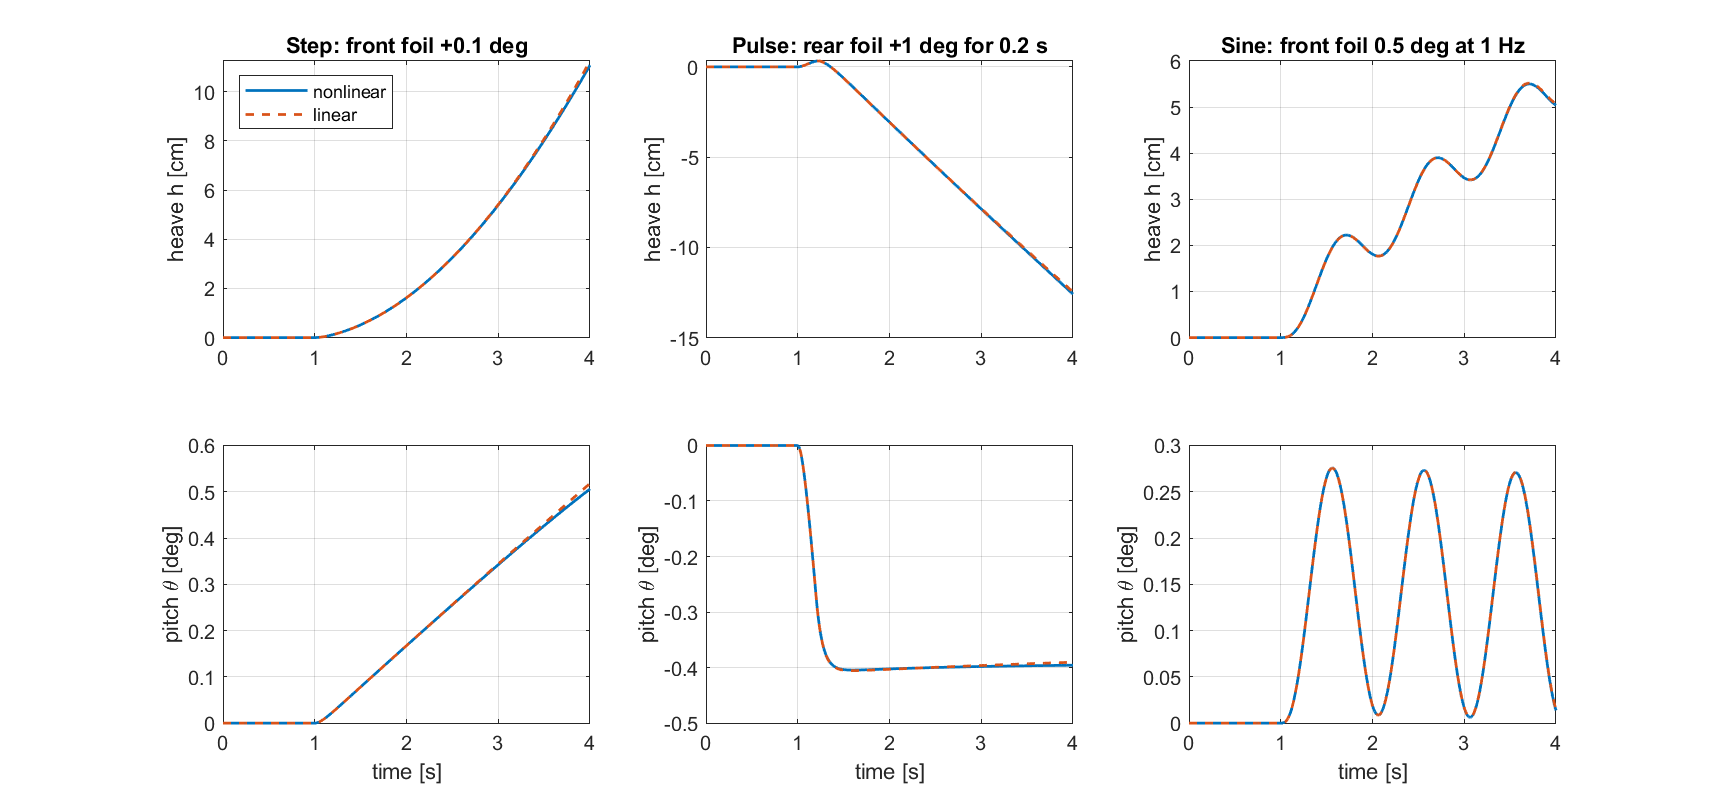
\includegraphics[width=\textwidth]{fig1_linear_vs_nonlinear.png}
\caption{Linear and nonlinear responses to a front-foil step, a rear-foil pulse
and a front-foil sine, all applied at $t=\SI{1}{s}$.}
\label{fig:sim1}
\end{figure}

\subsection{Range of validity of the linear model}

Figure~\ref{fig:sim2} repeats the front-foil step with increasing size. The two
models agree until the heave reaches about \SI{15}{cm}. Beyond that the foils
approach the surface, the free-surface factor $K$ falls quickly, and the
nonlinear model levels off at 24--\SI{27}{cm} while the linear model keeps
climbing. The model has no ventilation, so the behaviour this close to the
surface is only indicative; in reality the foils would be likely to ventilate
and lose more lift. We take the linear model as adequate for
$|h|\lesssim\SI{15}{cm}$, and the controller will have to keep the boat in that
range.

\begin{figure}[htbp]
\centering
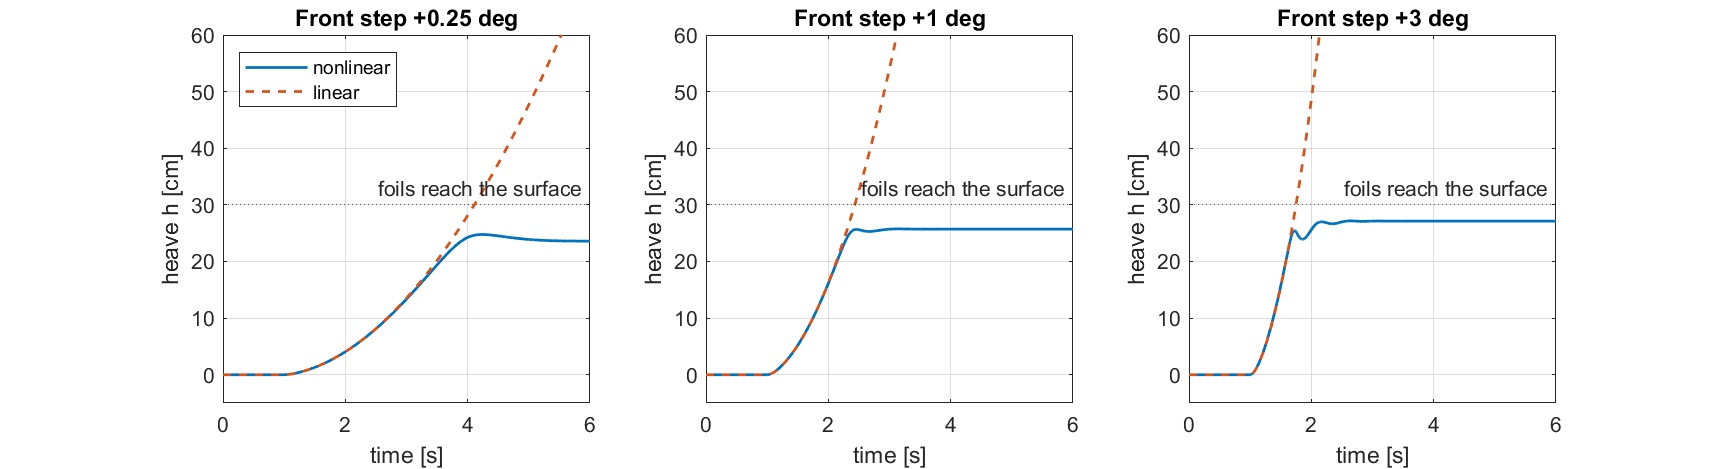
\includegraphics[width=\textwidth]{fig2_validity_range.png}
\caption{Front-foil steps of \SI{0.25}{\degree}, \SI{1}{\degree} and
\SI{3}{\degree}. The dotted line marks the height at which the foils reach the
surface.}
\label{fig:sim2}
\end{figure}

\subsection{Actuator constraints}

In Figure~\ref{fig:sim3} the front foils are commanded \SI{5}{\degree} above
trim, beyond the \SI{3.5}{\degree} that the mechanical limit allows. The applied
angle stops at \SI{7}{\degree} and takes about \SI{0.17}{s} to get there because
of the rate limit. The height response is delayed by about \SI{0.15}{s}. The
upward margin of \SI{3.5}{\degree} is therefore the binding constraint whenever
the controller needs more lift, for example to recover from a drop.

\begin{figure}[htbp]
\centering
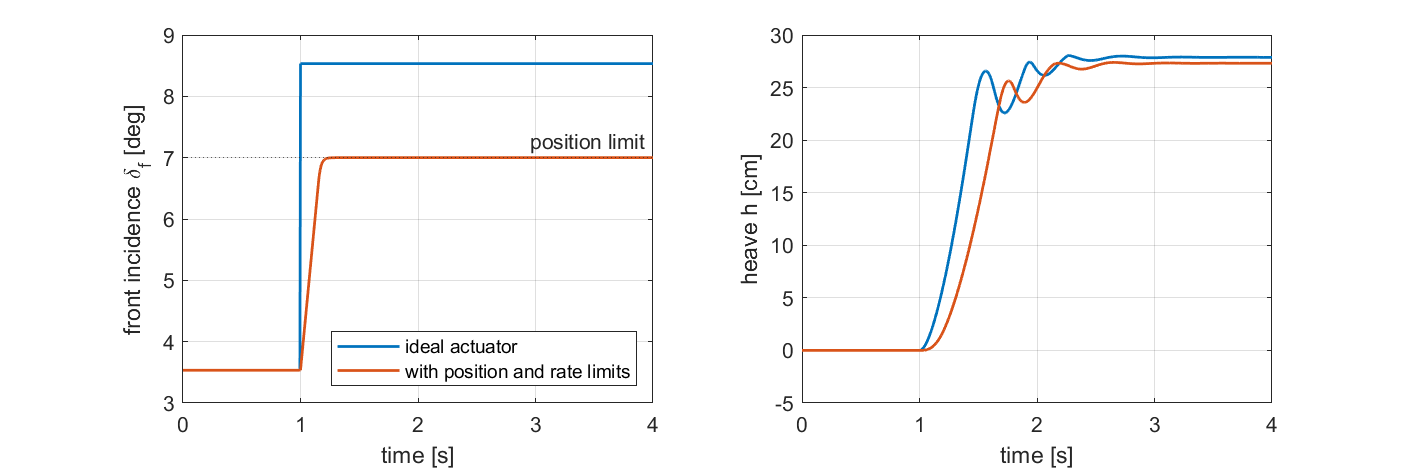
\includegraphics[width=0.85\textwidth]{fig3_actuator_limits.png}
\caption{A front-foil command beyond the position limit, with an ideal actuator
and with position and rate limits.}
\label{fig:sim3}
\end{figure}

\subsection{Model uncertainty}

Figure~\ref{fig:sim4} keeps the foils at the nominal trim incidences while the
true speed or mass differs from the design values. A speed error of
\SI{0.2}{m/s} (about \SI{3}{\percent}) moves the boat by about \SI{20}{cm} in
\SI{8}{s}; a mass error of \SI{10}{kg} (about \SI{5}{\percent}) by about
15--\SI{17}{cm}. A fixed trim setting cannot hold the ride height under
realistic parameter errors, so the controller will need integral action.

\begin{figure}[htbp]
\centering
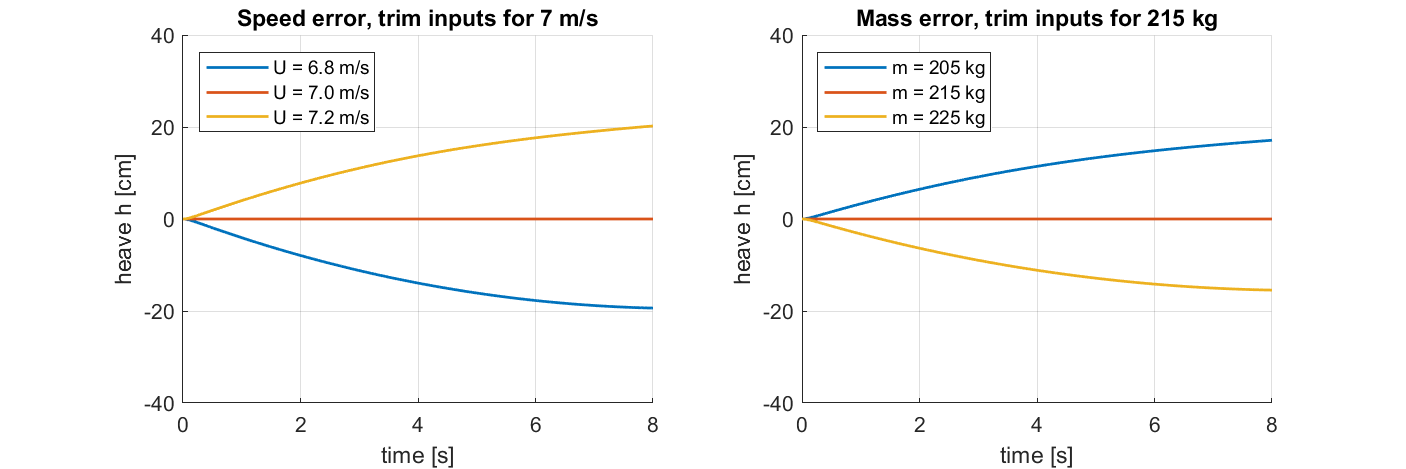
\includegraphics[width=0.85\textwidth]{fig4_uncertainty.png}
\caption{Heave with the inputs fixed at the nominal trim, for speed errors
(left) and mass errors (right).}
\label{fig:sim4}
\end{figure}

\subsection{Waves and measurements}

Figure~\ref{fig:sim5} shows the response to a regular head sea with amplitude
\SI{5}{cm} and wavelength \SI{8}{m}. At \SI{7}{m/s} the encounter frequency is
\SI{8.27}{rad/s} (\SI{1.32}{Hz}) and the vertical water velocity at foil depth
has an amplitude of \SI{0.11}{m/s}. The pitch angle oscillates by about
$\pm\SI{0.36}{\degree}$, and the heave oscillates while drifting upward; the
linear and nonlinear models separate once the drift exceeds about
\SI{15}{cm}, as in Figure~\ref{fig:sim2}.

The right panel shows the bow height that the ultrasonic sensor would report.
The wave surface passing under the bow and the sensor noise are of the same size
as the boat motion itself. The measurement cannot be fed back directly; it has
to be filtered by an observer.

\begin{figure}[htbp]
\centering
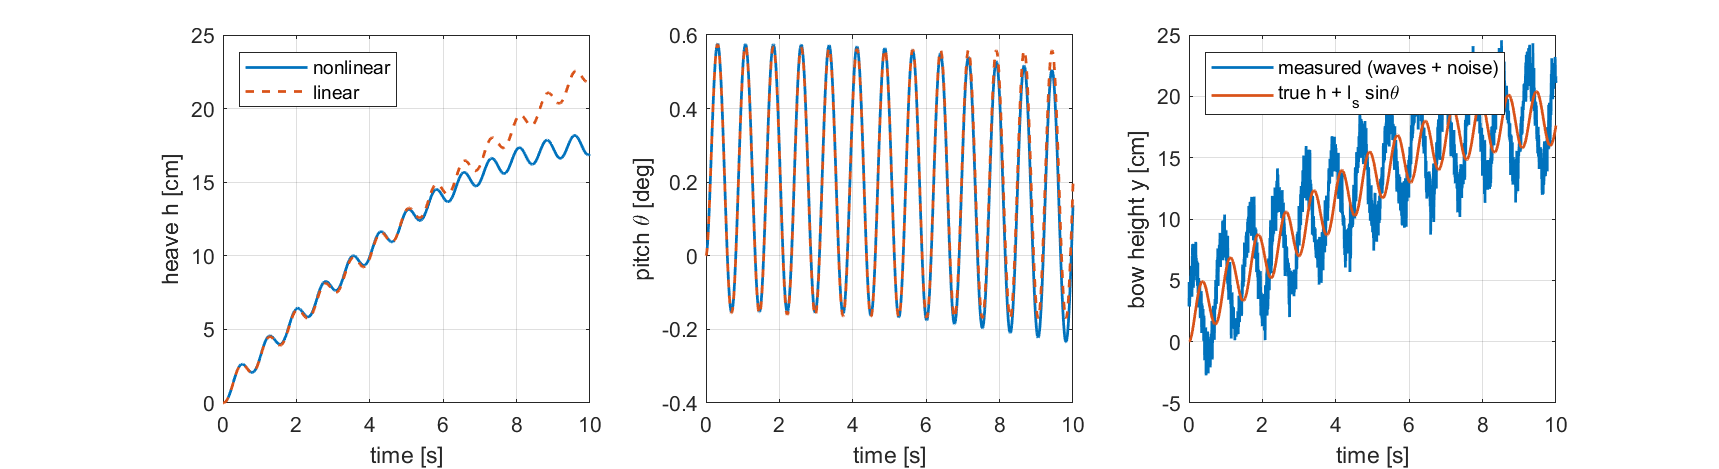
\includegraphics[width=\textwidth]{fig5_waves_and_sensor.png}
\caption{Regular head waves, no control: heave, pitch, and the measured bow
height compared with the true value $h+l_s\sin\theta$.}
\label{fig:sim5}
\end{figure}

\subsection{Complete Simulink model}

Figure~\ref{fig:sim6} runs the Simulink model with all effects enabled:
actuator limits, waves and sensor noise, and a \SI{1}{\degree} downward pulse
on the front foils lasting \SI{0.2}{s}. The applied angle lags the command
because of the servo lag and the rate limit. The linear and nonlinear heave stay
within a few millimetres of each other over the three seconds shown.

\begin{figure}[htbp]
\centering
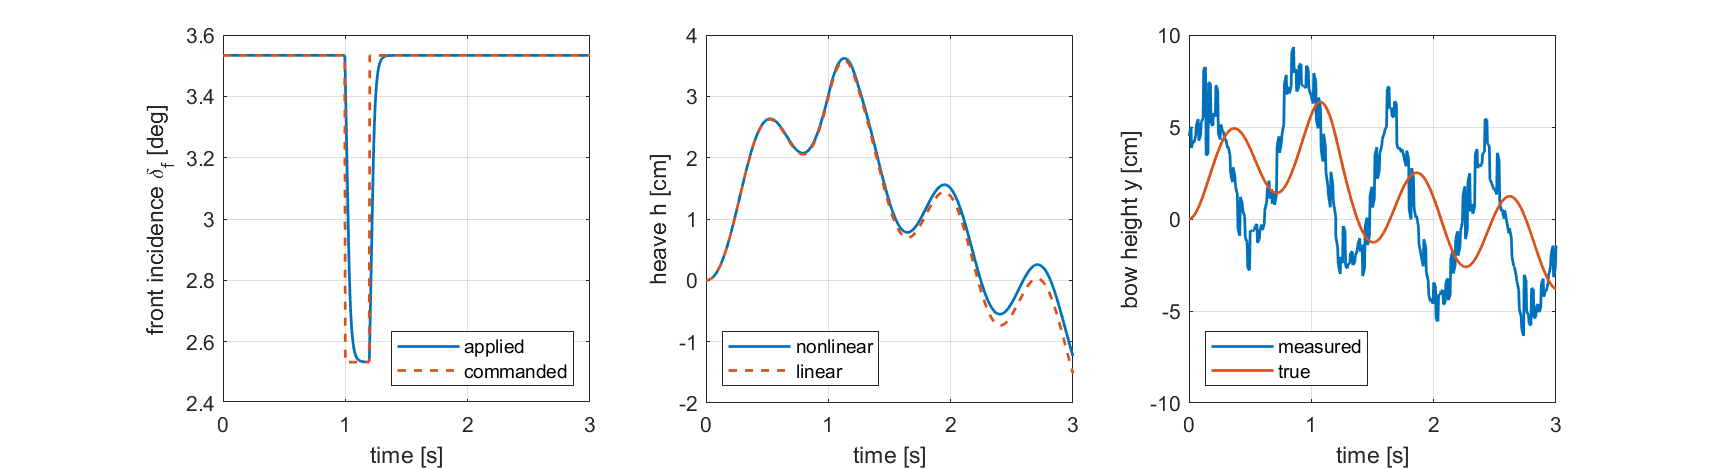
\includegraphics[width=\textwidth]{fig6_simulink_demo.png}
\caption{Simulink model with actuator limits, waves and sensor noise:
commanded and applied front-foil angle, heave, and measured bow height.}
\label{fig:sim6}
\end{figure}

\section{Limitations of the model}

The LTI model is valid for small deviations about level flight at one speed. It
does not represent take-off and landing, surge dynamics, unsteady (Theodorsen)
lift, downwash of the front foils on the rear foil, or foil ventilation. The
nonlinear model of Section~4, with saturation, rate limits, stall and sensor
noise, is used in simulation (Section~\ref{sec:sim}) and will be used to test the
controller outside the linear range.

\appendix
\section{Derivation of the free-surface factor}
\label{app:K}

At high Froude number gravity has no time to act on the free surface, and the
linearised free-surface condition reduces to zero velocity potential on the
undisturbed surface. This condition is met by placing an image of the foil at the
same distance $d$ above the surface, with circulation of the \emph{same} sense
(a rigid wall would require the opposite sense). The foil and its image form a
biplane with gap $2d$.

Represent the foil by a single bound vortex of circulation $\Gamma$ at the
quarter-chord point and enforce flow tangency at the three-quarter-chord point, a
distance $c/2$ downstream. The downwash there is the sum of the contributions of
the foil vortex and of the image vortex, which lies $c/2$ upstream and $2d$ above:
\[
\frac{\Gamma}{2\pi\,(c/2)} \;+\; \frac{\Gamma}{2\pi}\,
\frac{c/2}{(c/2)^2+(2d)^2} \;=\; U\alpha .
\]
Solving for $\Gamma$ and dividing by the deep-water value
$\Gamma_\infty=\pi c\,U\alpha$ gives
\[
K=\frac{\Gamma}{\Gamma_\infty}
 =\frac{1}{1+\dfrac{c^2}{c^2+16d^2}}
 =\frac{1+16\,(d/c)^2}{2+16\,(d/c)^2},
\]
which is \eqref{eq:K}. Since lift is proportional to circulation, the same factor
multiplies the lift. The result assumes a two-dimensional thin foil, small angle
of attack and infinite Froude number; it does not model ventilation.

\begin{thebibliography}{9}
\bibitem{belime} B.~J.~Belime, \emph{An hydrofoil control system for the SR02
vessel in the scope of the T\'ecnico Solar Boat Project}, MSc thesis, Instituto
Superior T\'ecnico, Universidade de Lisboa, October 2020.
\bibitem{renyang} J.~Ren and Y.~Yang, ``Fuzzy gain scheduling attitude control
for hydrofoil catamaran,'' in \emph{Proc.\ American Control Conference}, Boston,
MA, 2004, pp.~1103--1108.
\bibitem{liu} H.~Liu, Y.~Fu and B.~Li, ``Study of the LQRY-SMC control method for
the longitudinal motion of fully submerged hydrofoil crafts,'' \emph{J.\ Mar.\
Sci.\ Eng.}, vol.~10, no.~10, 1390, 2022.
\bibitem{faltinsen} O.~M.~Faltinsen, \emph{Hydrodynamics of High-Speed Marine
Vehicles}. Cambridge University Press, 2005, ch.~6.
\end{thebibliography}

\end{document}
